\chapter{Introducción}
\label{ch:intro}

\noindent Cualquier capítulo puede tener múltiples apartados, como el \autoref{sec:apartado1} o el \autoref{sec:sección2} de este mismo capítulo.

También está el \autoref{sec:ch2_1} del \autoref{ch:dos} que tiene la \autoref{fig:other}.

Es buena idea usar \texttt{\textbackslash{noindent}} al principio del primer párrafo, tras el encabezado de una sección o capítulo, para desactivar la sangría temporalmente.

\section{Listas de elementos}
\label{sec:apartado1}

\noindent Esta la lista de elementos del \autoref{sec:apartado1}:

\begin{itemize}
    \item Item 1
    \begin{itemize}
        \item Item 1
        \item Item 2
        \item Item 3
        \item Item 4
    \end{itemize}
    
    \item Item 2
    \item Item 3
    \item Item 4
\end{itemize}

\section{Enumeraciones}
\label{sec:sección2}

\noindent Esto es una lista enumerada, que puede estar relacionada con la \autoref{fig:intro}

\begin{enumerate}
    \item Item 1
    \begin{enumerate}
        \item Item 1
        \item Item 2
        \item Item 3
    \end{enumerate}
    \item Item 2
    \item Item 3
\end{enumerate}

\section{Figuras y tablas}

\noindent En la \autoref{fig:intro} se puede ver una figura de ejemplo. Las tablas, las figuras y los algoritmos (ver el \autoref{Apendice1:ZZZ}) son flotantes. Esto quiere decir que \LaTeX{} los intentará ubicar en el mejor lugar posible al componer el documento, intentando respetar ciertas reglas tipográficas. Como este lugar puede ser diferente a la posición que realmente ocupan en el texto, \textbf{es importante referenciar en el texto todas las figuras y las tablas}, en los diferentes puntos donde se hable de ellas.

\begin{figure}[htbp]
   \centering
   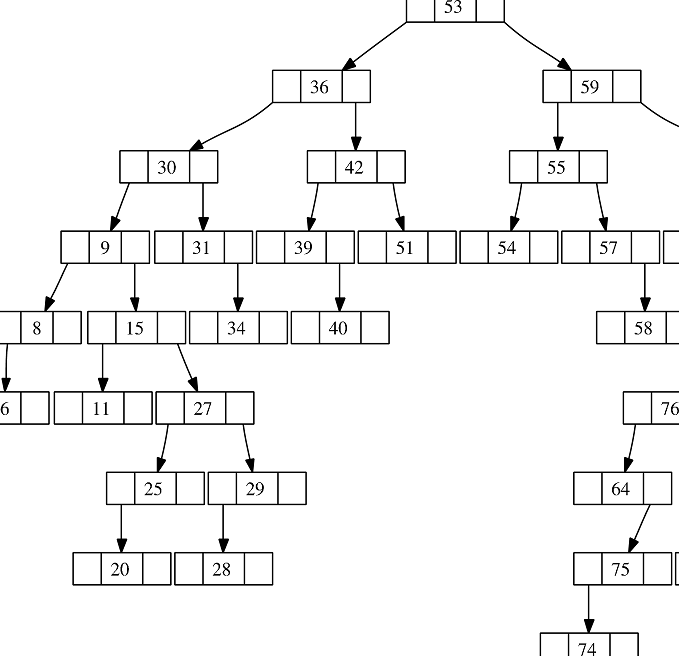
\includegraphics[width=0.8\linewidth]{images/figura_1}
   \caption{Ejemplo de figura.}
   \label{fig:intro}
\end{figure}

La \autoref{tbl:presupuesto} en el \autoref{ch:presupuesto} es un ejemplo de tabla hecha con el paquete \texttt{tabularx}.

Al crear tablas, figuras u otros elementos flotantes es aconsejable indicar siempre los especificadores de ubicación \texttt{[htbp]}, tal y como se hace en los ejemplos de esta plantilla. De esta forma \LaTeX{} intentará primero ponerlos en el lugar; si no puede, intentará ponerlos en la parte superior o inferior de la misma página y, en caso extremo, los pondrá en páginas especiales que solo contienen flotantes.

No es buena idea usar especificadores como \texttt{[h!]} o \texttt{[H]} para forzar una ubicación determinada. El motivo es que eso impide a \LaTeX{} buscar la mejor forma de componer el documento, pudiendo dar como resultado páginas que se ven muy raras --por ejemplo, dejando muchos huecos libres entre el texto--.

\section{Código y algoritmos}

\noindent En el \autoref{apx:1} se pueden observar varios ejemplos de entornos para describir algoritmos y código.

\section{Citas}

\noindent Las referencias bibliográficas se deben indicar en el archivo \texttt{references.bib} y se citan en el texto. Las referencias no citadas no aparecerán en el apartado de la bibliografía.

Las citas pueden ser entre paréntesis \parencite{examplearticle} o \emph{en línea}, como la de \cite{examplegithub}.

Las  reglas para citar \parencite{ulllibguide} permiten citar cualquier cosa: artículos de investigación, libros, entradas de la Wikipedia, blogs, vídeos de Youtube o repositorios de GitHub, entre otros. 

En el \autoref{ch:cuatro} se puede ver otro tipo de citas, usando el paquete \texttt{csquotes}, donde se traslada de forma literal una porción del texto original al documento.
 
\section{Otra sección...}

\noindent \lipsum[1]

\subsection{Con subsección...}

\noindent \lipsum[2]